\documentclass[12pt]{article}
\pdfminorversion=7

% Standard packages for figures, citations, math, tables, etc.
% Feel free to add more as needed!
\usepackage{amssymb}
\usepackage{graphicx}
\usepackage{cite}
\usepackage[cmex10]{amsmath}
\interdisplaylinepenalty=2500 
\usepackage{mdwmath}
\usepackage{mdwtab}
\usepackage{color}
\usepackage{pgfplots}
\usepackage{multirow}
\usepackage{subcaption}
\usepackage{verbatim}
\usepackage{appendix}
\usepackage[outdir=./]{epstopdf}
\usepackage{indentfirst}
\pgfplotsset{compat=1.17}

% Packages for formatting with 1 in margins
\usepackage[latin1]{inputenc}
\usepackage[left=1in,top=1in,right=1in,bottom=1in,nohead]{geometry}
\usepackage{setspace}
\setstretch{1.15}
\setlength\parindent{1cm}

% Define the location of your figures in order to avoid writing absolute file location
\graphicspath{{figures/}}	

\begin{document}

% Title Page
\begin{titlepage}
\begin{center}
{\LARGE \textsc{ECE 445: Senior Design Laboratory} \\ \vspace{8pt}}
\rule[13pt]{\textwidth}{1pt} \\ \vspace{120pt}
{\huge \textbf{\textsc{The Odds Booster}} \\ \vspace{8pt}}
{\LARGE \textbf{\textsc{Project Proposal}} \\ \vspace{30pt}} 
{\large \textit{Authors:} Marco Rojas \\ \vspace{4pt}
\hspace{48pt} Jack Arndt \\ \vspace{4pt}
\hspace{48pt} Tim Green \\ \vspace{4pt}
\hspace{8pt} \textit{Date Written:} February 9th, 2022}
\vfill
\end{center}

% Numbered pages on everything but title
\pagenumbering{arabic}	
\end{titlepage}
\setcounter{page}{2}

% Body
\section{Introduction}

Before heading to the casino, individuals need to assess how much money they are willing to lose, since, as the saying goes, ``The house always wins''. Or do they? Is there potentially a way to bring the casino games to the comfort of your home and train/optimize your strategies to ask a different question, ``How much money should I win?''

The Odds Booster is an automated casino game assistant designed to help players learn and manage casino games such as Blackjack or Texas Hold'em. The kit involves a central communicable device along with a custom deck of cards which will be used to determine the best possible move for each player along with the outcome of each hand of the game. This device is an innovation as it brings both the ease and simplicity as well as the ability to learn the game that can be provided by a virtual game into the superior enjoyment and atmosphere of a physical game. Digital poker tables that provide a similar experience exist but cost thousands of dollars. Our design achieves this functionality without an expensive custom table and while allowing for physical cards and chips.

The Odds Booster central device will serve as the hub used by the dealer and all players of the game. The dealer will swipe each card being distributed to the players over the central device and said device will determine the specific card being dealt using an RFID sensor and thin passive RFID tags placed on the cards. This central device will also contain a display detailing the next actions and outcomes for each hand of the game helping each player and the dealer learn the rules of the game. This main device will be paired via bluetooth to a user's phone app. The card information will be shared with the app and the app will tell the player the strength of their hand or what move will have the best outcome within the context of the game. It is important to note that knowledge of the hands of the other players within the game provides an unfair advantage to the user and such information will be ignored when determining moves for the user. The ethics of the game will be discussed further later in this proposal. The device itself will be battery powered and rechargeable for easy use and mobility. The usage of the device is protrayed in the diagram shown in Figure \ref{fig:use_dia}.

\begin{figure}[h!]
	\centering
	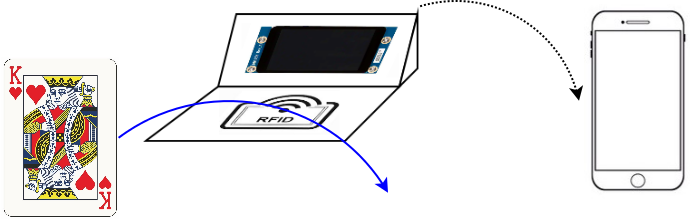
\includegraphics[width=0.9\textwidth]{ProposalUsageDiagram.png}
	\caption{System Usage Diagram}
	\label{fig:use_dia}
\end{figure}

\noindent
The main requirements to ensure the completion and success of this project are as follows.
\begin{itemize}
\item The central device must be able to sense and distinguish the 52 different RFID tags associated with each card.
\item The central device must be able to display the card and game information for all players to see as well as send the information to a phone app via bluetooth.
\item The phone app must be able to receive game information via bluetooth and use the information to determine the strength of the user's hand and/or the best possible move for the user.
\end{itemize}
These requirements are broken into more detailed and module specific requirements through the remainder of this proposal.

\section{Design}

The block diagram describing each module within the system and their connections is shown in Figure \ref{fig:block}. The design is composed of five main modules or subsystems. Four of the modules are outlined by hardware components and labeled in the block diagram. The fifth module is the phone app. The purpose, interconnections, and requirements of each module are described in detail through this section. The requirements specified in this proposal give an idea of the standards to which we will hold our design, but do not provide testing methods at this time.

\begin{figure}[h!]
	\centering
	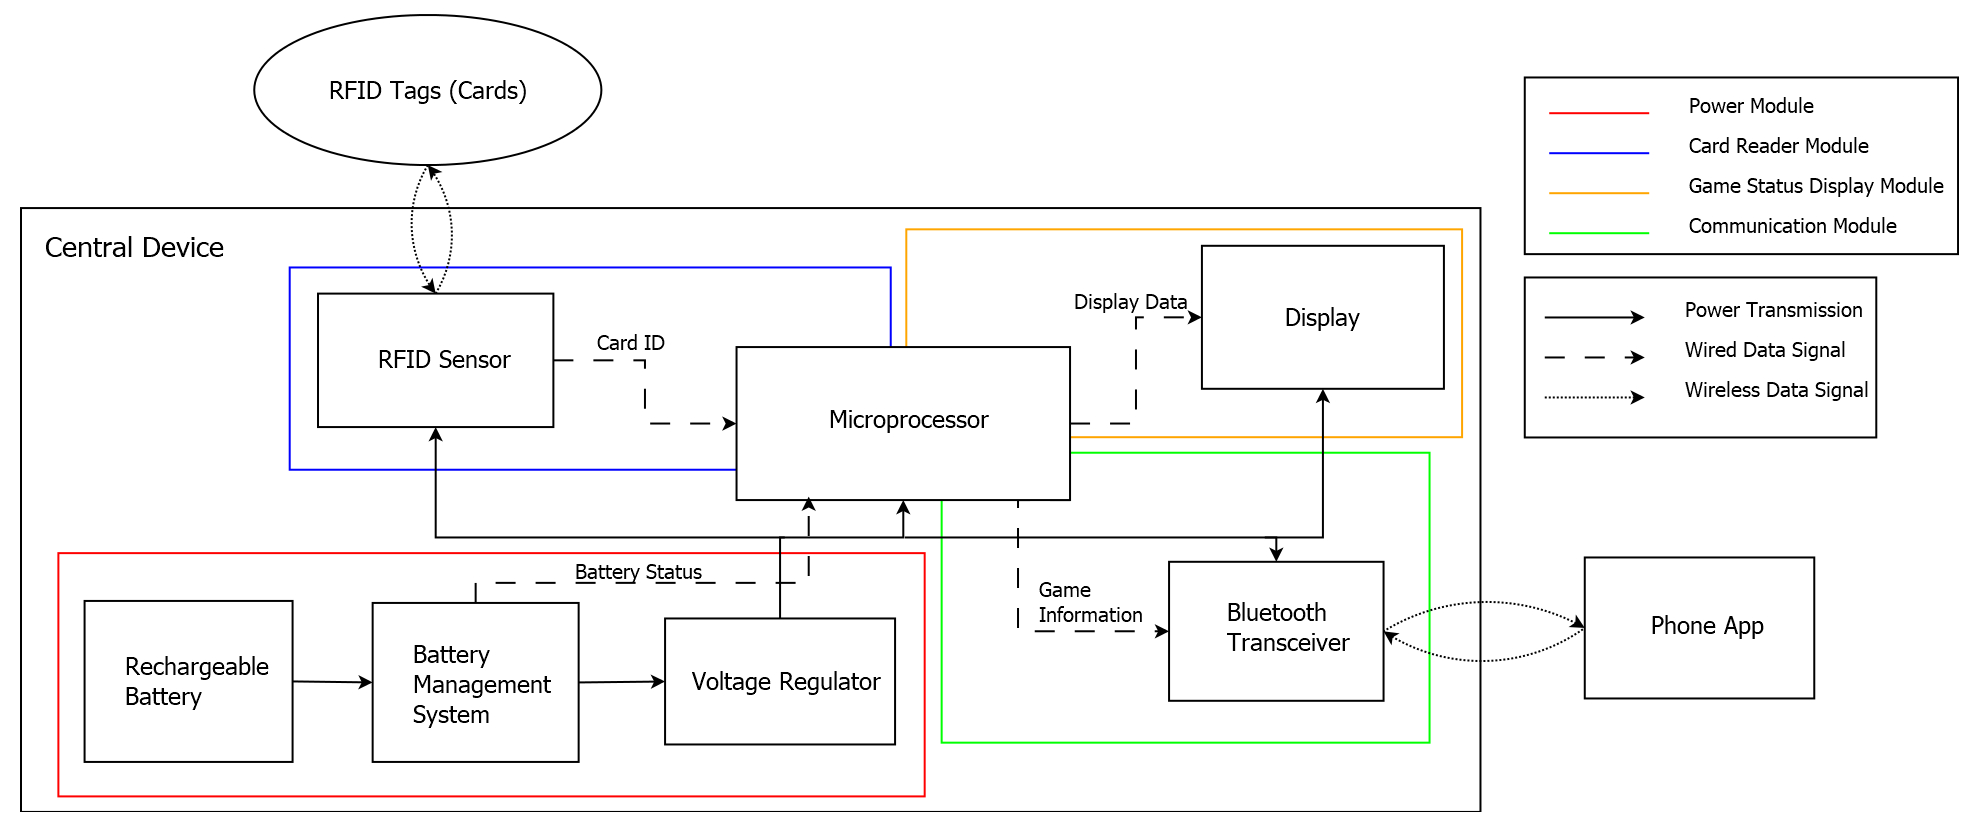
\includegraphics[width=0.98\textwidth]{Full_Block_Diagram_v3.png}
	\caption{Block Diagram}
	\label{fig:block}
\end{figure}

\subsection{Power Module}

The power module is made up of a rechargeable battery, a battery management system, and a voltage regulator. This module is responsible for providing power to all other hardware components within the system in a safe manner. Without this module, none of the main requirements could be met as each operation of the system requires power. The power module connects to the other three hardware modules (the card reader, game status display, and communications modules) via a DC voltage provided by the voltage regulator. This DC voltage is dependent on requirements set by specific component models but is likely to be $3.3V$ as this is the nominal operating voltage for most CMOS devices. The battery management system also connects to the game status display module as it provides the microprocessor with battery status information. This signal is used to tell the users important system information such as when the battery is low.

The rechargeable battery will be a lithium ion battery. This is a popular rechargeable battery that tends to have  good energy and power density. More research will be needed on expected power draw to determine the battery capacity sizing. The lithium ion battery output will be connected to a battery management system. The battery management system (BMS) is used to monitor the status of the battery in terms of output voltage and current draw. This protects the battery from being over or undercharged and from being overdrawn by being able to cut power connections. This allows for a longer battery life and a safer device. The BMS is then connected to the voltage regulator. The voltage regulator ensures the voltage of the battery remains at a safe level for each component in the system.

The power module has a set of basic requirements that ensure its proper operation. These requirements are as follows.

\begin{itemize}
\item The battery management system must be able to measure the output voltage of the lithium ion battery to a tolerance of $\pm0.1V$.
\item The battery management system must be able to measure the current in or out of the lithium ion battery to a tolerance of $\pm10mA$.
\item The battery management system must be able to disconnect connected components if the lithium ion battery voltage falls too low or moves too high (specific boundaries depend on specific battery model safety specifications).
\item The voltage regulator must be able to maintain a voltage within a safe range of $3.1V$ to $3.5V$ (safe operating range for average CMOS device \cite{TI_inverter}).
\item The power must be able to continously provide at least $500mA$ given the voltage regulator requirements
\end{itemize}

\subsection{Card Reader Module}

The card reader module is made up of the microprocessor and the RFID sensor. The module is responsible for reading the card ID of each card swiped past the device. The module is vital for the first main requirement of sensing and distinguishing each of the 52 cards. The card reader module connects to the power module through the provided $3.3V_{DC}$ supply, and to the game status display and communication modules through the passing of data within the microprocessor.

The RFID sensor generates a specific frequency signal that powers the RFID tags on the cards and results in the cards transmitting a signal containing the serial ID of the tag. The frequency of the sensor depends on the selected RFID tags operating frequency. The microprocessor is shared by multiple modules but will receive this serial ID from the sensor via wired serial transmission.

The basic requirements for the card reader module that ensure its proper operation are as follows.

\begin{itemize}
\item The RFID sensor must be able to accurately determine the serial ID of an RFID tag when held to the surface of the sensor.
\item The microprocessor must be able to accurately receive the serial ID of the RFID tag when serially transmitted from the RFID sensor.
\end{itemize} 

\subsection{Game Status Display Module}

The game status display module is made up of the microprocessor and the display. The module is responsible for showing the user the game actions and current game information. The module is vital for the second main requirement in displaying to the players and dealer the game status and next actions. The game status display module connects to the power module through the DC supply, and the card reader module through the transfer of card data within the microprocessor.

The display within the module is an output device showing the video data provided to it by the microprocessor. As the microprocessor must be able to provide video data to the display via a VGA protocol, the output capabilities of the microprocessor must be high enough to transfer information to the display at a fast enough rate. The microprocessor must also have enough memory to hold the necessary sprites and potentially a screen buffer (depending on the display size and control method used).

The basic requirements for the game status display module that ensure its proper operation are as follows.

\begin{itemize}
\item The display must be able to show the next action of the game at any given time in the form of text on the screen.
\item The microprocessor must be able to transmit the video data through VGA protocol to the display at a standard rate of $\sim30$fps.
\end{itemize}

\subsection{Communication Module}

The communication module is made up of the bluetooth transceiver and the microprocessor. The module is repsonsible for communicating the card and game data from the central device to the phone app as well as receiving information from the phone app. The module is vital for the second and third main requirements in sending the game data and allowing the use of this data within the phone app. The communication module connects to the power module through the DC supply, to the card reader module through the transfer of card data within the microprocessor, and to the phone app through a 2.4GHz wireless signal.

The bluetooth transceiver is used to generate a 2.4GHz signal (bluetooth protocol frequency) to send card information to the phone app. Likewise, the transceiver receives similar frequency signals and send the signal data to the microprocessor for use by the system in setting game status. The microcontroller will generate the bluetooth packet for use by the transceiver and will follow normal bluetooth protocol in its operation to ensure compatibility with many devices.

The basic requirements for the communication module that ensure its proper operation are as follows.

\begin{itemize}
\item The microprocessor must follow the bluetooth protocol as specified in \cite{IEEE_bt}.
\item The communication module must be able to communicate with a device at a distance of 3ft with an average thoughput of 10kbps (small amount of data transfer does not require high throughput).
\end{itemize}

\subsection{Phone App Module}

The phone app module is made up of solely the application used by the phone. The module is responsible for receiving the communications from the central device and sending control information back to the device. The module is vital for the third main requirement in the receipt of game data by the phone and display of optimal moves or game statistics. The phone app module connects only to the communication module in the wireless transmission of game information.

The phone app relies on the device having bluetooth capabilities. The app receives game data and uses statistics and probability methods to determine the strength of the users hand in relation to other possible hands within the game. The app displays this measurement to the user and will use this strength measure to suggest moves to the user. With enough time and successful work, the app could potentially use a machine learning algorithm to continue to provide better suggestions with more use. 

The basic requirements for the phone app module that ensure its proper operation are as follows.

\begin{itemize}
\item The app must be able to utilize the bluetooth capabilities of the device to successfully send and receive data with the central device.
\item The app must be able to use information to accurately calculate the ``strength'' measure. This measure consists of comparing the current hand of the user to all other possible hands and determine the ranking percentile. (More specific measures may be provided depending on game type).
\item The app must be able to display the measures and suggestions in the form of text for the user.
\end{itemize}

\section{Ethics and Safety}

Gambling and wagering money on casino games inherently raises an ethics-eyebrow. Getting involved in this space requires the ability to tread lightly and ensure the IEEE Code of Ethics \cite{IEEE_ethics} is followed to a tee. While our project is aimed at improving players' abilities to perform in the casino, there are measures that need to be accounted for during the development of this project and issues that could potentially arise from accidental or intentional misuse of our project. 

First, we must acknowledge what are the common laws that are broken when cheating in the casino. NRS 465.083 \cite{NRS}, according to Nevada law, prohibits players from cheating at a casino game, which by definition is the manipulation of the outcome of the game or the payments made. This can lead to a felony charge, with 1 to 5 years in prison, restitution, and up to \$10,000 in fines. Essentially, this is a fraud charge specifically citing it happening in the casino. The legal definition is stated as ``alter[ing] the elements of chance, method of selection, or criteria which determine'' the results, amount of payment, or frequency of payment in a game \cite{NRS}; This relates to IEEE Code of Ethics I.4 \cite{IEEE_ethics}. In order to avoid ethical breaches, we are requiring that the usage of our project will have all casino cards scanned and in need of compliance with the dealer. Any dealer that is sitting at a table game in the casino will clearly not agree to use our project as it's in clear violation of casino policy, and even with a dealer that is in cahoots with the player will immediately be caught with the ``Eyes in the Sky'' which is the term for the security measures in the casino. Essentially, we are taking the route that there is no lowkey or secretive way to use this device in the casino that you wouldn't get caught trying to use outside resources to help boost your odds and chances of winning. A custom deck of cards and a table-top card scanner is impossible to get by the security systems at the casino. 

Next, we look into the potential harm that this project can deliver to the players and general public. This relates to IEEE Code of Ethics I.1 \cite{IEEE_ethics}, and due to our planned usage of RFID and Bluetooth technologies, we are not transmitting or receiving any harmful signals that are outside the typical broadband spectrum of frequencies. There will be no cause of concern for the wireless communications occurring throughout the usage of this project. According to the FDA, there is no evidence of any adverse effects associated with the usage of passive RFID \cite{FDA_RFID}.

Furthermore, IEEE Code of Ethics I.3 \cite{IEEE_ethics} references conflicts of interest, which could potentially pertain to the casinos and their disliking to players increasing their odds of winning. Since this is purely an educational tool, there should be no issues with the casinos and the usage of this in the casino proper is virtually impossible thanks to our design of the project and tight security measures that are relevant to every casino.

Since our project does not in any way put others down or engage in any sort of harassment or discrimination, the IEEE Code of Ethics II \cite{IEEE_ethics} is fulfilled as well. 

Lastly, taking a quick look at the Bluetooth Code of Conduct \cite{BT_conduct} will show that we are following each item and staying true to the ethics laid out. We are not violating any law, transmitting harmful content or tampering, or sending excessively high volume data transfers or bandwidth consumption.

Ethical breaches are primarily prevented due to the design of our project, which requires the usage of a table-top card scanner and our own custom deck of cards (which obviously can not be used in the casino). Players are unable to use the Odds Booster if the custom deck of cards isn't being used, since it's the way that players are able to know what the best possible choices are to take in the casino games. The card scanner needs to send the information to the phone app to crunch the data, thereby preventing the use of any other cards. 

As with any design project, there will always be safety concerns that need to be acknowledged, assessed, and accounted for. In the following section, these concerns are discussed with respect to their associated hazards and potential solutions to minimize any possibilities of risk.

Typically, the primary point of safety concern for any electrical system design stems from the source of power. The power source is not only responsible for the system's overall functionality, but can also work to destroy necessary hardware components (or modules) due to unanticipated variations in power output. To take this into account, our power module consists of a rechargeable battery, a battery management system, and a voltage regulator. As specified in greater detail in the Power Module section, the battery management system and voltage regulator ensure the system's overall immunity to variations in current and voltage such that each individual component can operate at a safe level. It is important to note that the rechargeable battery being used is a lithium ion battery. As per the ECE 445 Safety Guidelines \cite{445_safety}, ``Any group charging or utilizing certain battery chemistries must read, understand, and follow guidelines for safe battery usage.'' All members of the group have read and agreed to follow the course staff's guidance regarding high capacity batteries \cite{Li_safety} and will complete all necessary safety training and adhere to the guidelines set forth in the aforementioned document. 

Before moving on, it is worth to note that the maximum voltage our system will operate under is approximately 3.3V - 3.6V. Inherently, we will be working with relatively low voltages and currents. This is reassuring to know that while we may not be as subject to the greater (and more dangerous!) risks posed from working with higher voltage equipment, that does not mean we can neglect basic lab and equipment safety policies and procedures. All members of the group have also completed the required lab safety training to gain access to the lab. 

Overall, this project is considered relatively ``safe'' under the context of adhering to proper safety policies and protocols when in the lab. There are no true significant safety concerns to the end user as well. The user will simply operate the device primarily from his/her phone and be isolated from any true risk of electrical or mechanical interaction as the entire system will be housed in a custom CAD-designed enclosure. This enclosure serves a double purpose in that it will shield the user/environment from exposure to the electrical components and vice versa. 

% Bibliography (references in separate file)
\bibliographystyle{IEEEtran}
\bibliography{references.bib}

% Appendix (If Applicable)

\end{document}
